\documentclass{standalone}
\usepackage{tikz}
\usetikzlibrary{patterns, positioning}
\usepackage[sfdefault]{ClearSans} %% option 'sfdefault' activates Clear Sans as the default text font
\usepackage[T1]{fontenc}

\begin{document}
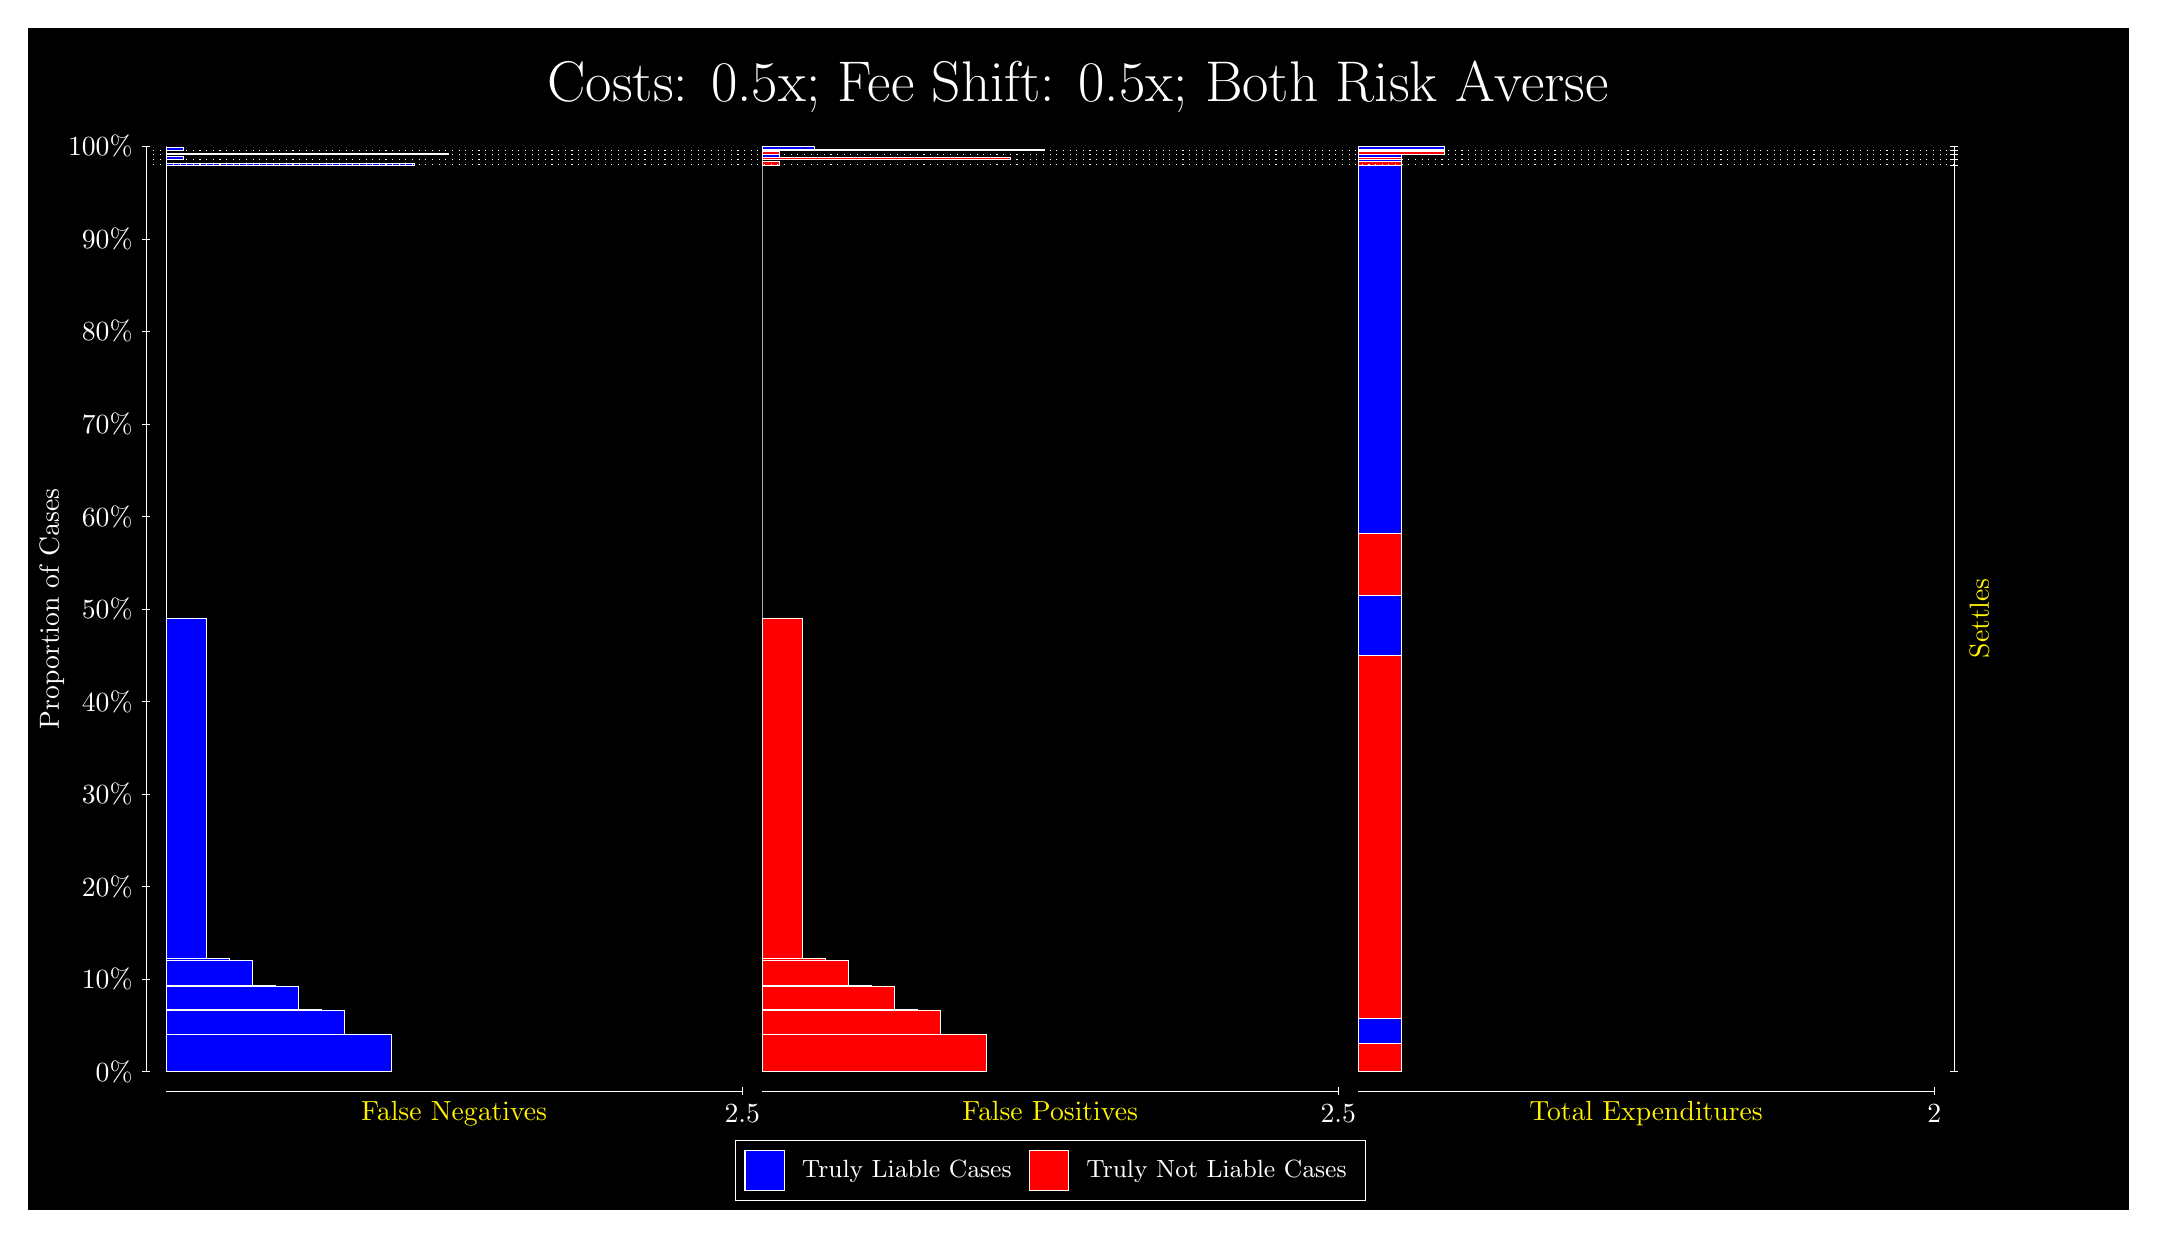
\begin{tikzpicture}
\draw[fill=black] (0,0) rectangle (26.667,15);
\draw[text=white] (0,13.5) rectangle (26.667,15) node[midway] {\huge Costs: 0.5x; Fee Shift: 0.5x; Both Risk Averse};
\draw[white, very thin] (1.5,1.75) -- (1.5,13.5);
\node[rotate=90, text=white, anchor=center] at (0.3, 7.625) {Proportion of Cases};
\draw[white, very thin] (1.45,1.75) -- (1.55,1.75);
\node[text=white, anchor=east] at (1.45, 1.75) {0\%};
\draw[white, very thin] (1.45,2.925) -- (1.55,2.925);
\node[text=white, anchor=east] at (1.45, 2.925) {10\%};
\draw[white, very thin] (1.45,4.1) -- (1.55,4.1);
\node[text=white, anchor=east] at (1.45, 4.1) {20\%};
\draw[white, very thin] (1.45,5.275) -- (1.55,5.275);
\node[text=white, anchor=east] at (1.45, 5.275) {30\%};
\draw[white, very thin] (1.45,6.45) -- (1.55,6.45);
\node[text=white, anchor=east] at (1.45, 6.45) {40\%};
\draw[white, very thin] (1.45,7.625) -- (1.55,7.625);
\node[text=white, anchor=east] at (1.45, 7.625) {50\%};
\draw[white, very thin] (1.45,8.8) -- (1.55,8.8);
\node[text=white, anchor=east] at (1.45, 8.8) {60\%};
\draw[white, very thin] (1.45,9.975) -- (1.55,9.975);
\node[text=white, anchor=east] at (1.45, 9.975) {70\%};
\draw[white, very thin] (1.45,11.15) -- (1.55,11.15);
\node[text=white, anchor=east] at (1.45, 11.15) {80\%};
\draw[white, very thin] (1.45,12.325) -- (1.55,12.325);
\node[text=white, anchor=east] at (1.45, 12.325) {90\%};
\draw[white, very thin] (1.45,13.5) -- (1.55,13.5);
\node[text=white, anchor=east] at (1.45, 13.5) {100\%};

\draw[white, very thin] (24.457,1.75) -- (24.457,13.5);
\draw[white, very thin] (24.407,1.75) -- (24.507,1.75);
\node[anchor=west] at (24.407, 1.75) {};
\draw[white, very thin] (24.407,13.265) -- (24.507,13.265);
\node[anchor=west] at (24.407, 13.265) {};
\draw[white, very thin] (24.407,13.332) -- (24.507,13.332);
\node[anchor=west] at (24.407, 13.332) {};
\draw[white, very thin] (24.407,13.398) -- (24.507,13.398);
\node[anchor=west] at (24.407, 13.398) {};
\draw[white, very thin] (24.407,13.449) -- (24.507,13.449);
\node[anchor=west] at (24.407, 13.449) {};
\draw[white, very thin] (24.407,13.5) -- (24.507,13.5);
\node[anchor=west] at (24.407, 13.5) {};

\draw[white, very thin, fill=blue] (1.75,1.75) rectangle (4.6044,2.2189);
\draw[white, very thin, fill=blue] (1.75,2.2189) rectangle (4.3116,2.2287);
\draw[white, very thin, fill=blue] (1.75,2.2287) rectangle (4.0188,2.5292);
\draw[white, very thin, fill=blue] (1.75,2.5292) rectangle (3.7261,2.539);
\draw[white, very thin, fill=blue] (1.75,2.539) rectangle (3.4333,2.8302);
\draw[white, very thin, fill=blue] (1.75,2.8302) rectangle (3.1406,2.8508);
\draw[white, very thin, fill=blue] (1.75,2.8508) rectangle (2.8478,3.1621);
\draw[white, very thin, fill=blue] (1.75,3.1621) rectangle (2.5551,3.1827);
\draw[white, very thin, fill=blue] (1.75,3.1827) rectangle (2.2623,7.5074);
\draw[white, very thin, fill=red] (1.75,7.5074) rectangle (1.75,13.265);
\draw[white, very thin, fill=blue] (1.75,13.265) rectangle (4.8971,13.289);
\draw[white, very thin, fill=red] (1.75,13.289) rectangle (1.75,13.332);
\draw[white, very thin, fill=blue] (1.75,13.332) rectangle (1.9696,13.374);
\draw[white, very thin, fill=red] (1.75,13.374) rectangle (1.75,13.398);
\draw[white, very thin, fill=blue] (1.75,13.398) rectangle (5.3362,13.417);
\draw[white, very thin, fill=red] (1.75,13.417) rectangle (1.75,13.449);
\draw[white, very thin, fill=blue] (1.75,13.449) rectangle (1.9696,13.482);
\draw[white, very thin, fill=red] (1.75,13.482) rectangle (1.75,13.5);
\draw[white, very thin, fill=red] (9.3189,1.75) rectangle (12.173,2.2189);
\draw[white, very thin, fill=red] (9.3189,2.2189) rectangle (11.88,2.2287);
\draw[white, very thin, fill=red] (9.3189,2.2287) rectangle (11.588,2.5292);
\draw[white, very thin, fill=red] (9.3189,2.5292) rectangle (11.295,2.539);
\draw[white, very thin, fill=red] (9.3189,2.539) rectangle (11.002,2.8302);
\draw[white, very thin, fill=red] (9.3189,2.8302) rectangle (10.709,2.8508);
\draw[white, very thin, fill=red] (9.3189,2.8508) rectangle (10.417,3.1621);
\draw[white, very thin, fill=red] (9.3189,3.1621) rectangle (10.124,3.1827);
\draw[white, very thin, fill=red] (9.3189,3.1827) rectangle (9.8312,7.5075);
\draw[white, very thin, fill=blue] (9.3189,7.5075) rectangle (9.3189,13.265);
\draw[white, very thin, fill=red] (9.3189,13.265) rectangle (9.5384,13.308);
\draw[white, very thin, fill=blue] (9.3189,13.308) rectangle (9.3189,13.332);
\draw[white, very thin, fill=red] (9.3189,13.332) rectangle (12.466,13.356);
\draw[white, very thin, fill=blue] (9.3189,13.356) rectangle (9.5384,13.398);
\draw[white, very thin, fill=red] (9.3189,13.398) rectangle (9.5384,13.431);
\draw[white, very thin, fill=blue] (9.3189,13.431) rectangle (9.3189,13.449);
\draw[white, very thin, fill=red] (9.3189,13.449) rectangle (12.905,13.467);
\draw[white, very thin, fill=blue] (9.3189,13.467) rectangle (9.9776,13.5);
\draw[white, very thin, fill=red] (16.888,1.75) rectangle (17.437,2.1025);
\draw[white, very thin, fill=blue] (16.888,2.1025) rectangle (17.437,2.4226);
\draw[white, very thin, fill=red] (16.888,2.4226) rectangle (17.437,7.0386);
\draw[white, very thin, fill=blue] (16.888,7.0386) rectangle (17.437,7.7987);
\draw[white, very thin, fill=red] (16.888,7.7987) rectangle (17.437,8.5877);
\draw[white, very thin, fill=blue] (16.888,8.5877) rectangle (17.437,13.265);
\draw[white, very thin, fill=red] (16.888,13.265) rectangle (17.437,13.308);
\draw[white, very thin, fill=blue] (16.888,13.308) rectangle (17.437,13.332);
\draw[white, very thin, fill=red] (16.888,13.332) rectangle (17.437,13.356);
\draw[white, very thin, fill=blue] (16.888,13.356) rectangle (17.437,13.398);
\draw[white, very thin, fill=red] (16.888,13.398) rectangle (17.986,13.431);
\draw[white, very thin, fill=blue] (16.888,13.431) rectangle (17.986,13.449);
\draw[white, very thin, fill=red] (16.888,13.449) rectangle (17.986,13.467);
\draw[white, very thin, fill=blue] (16.888,13.467) rectangle (17.986,13.5);
\draw[white, dotted] (1.5,13.265) -- (24.457,13.265);
\draw[white, dotted] (1.5,13.332) -- (24.457,13.332);
\draw[white, dotted] (1.5,13.398) -- (24.457,13.398);
\draw[white, dotted] (1.5,13.449) -- (24.457,13.449);
\draw[white, very thin] (1.75,1.5) -- (9.0689,1.5);
\node[text=yellow, anchor=north] at (5.4094, 1.5) {False Negatives};
\draw[white, very thin] (9.0689,1.45) -- (9.0689,1.55);
\node[text=white, anchor=north] at (9.0689, 1.45) {2.5};

\draw[white, very thin] (9.3189,1.5) -- (16.638,1.5);
\node[text=yellow, anchor=north] at (12.978, 1.5) {False Positives};
\draw[white, very thin] (16.638,1.45) -- (16.638,1.55);
\node[text=white, anchor=north] at (16.638, 1.45) {2.5};

\draw[white, very thin] (16.888,1.5) -- (24.207,1.5);
\node[text=yellow, anchor=north] at (20.547, 1.5) {Total Expenditures};
\draw[white, very thin] (24.207,1.45) -- (24.207,1.55);
\node[text=white, anchor=north] at (24.207, 1.45) {2};

\node[text=yellow, centered, rotate=90] at (24.777, 7.5074) {Settles};





\draw (12.978300999999998,1.5) node[draw=none] (baseCoordinate) {};
\begin{scope}[align=center]
        \matrix[scale=0.5, draw=white, below=0.5cm of baseCoordinate, nodes={draw}, column sep=0.1cm]{
            \node[rectangle, draw, minimum width=0.5cm, minimum height=0.5cm, fill=blue] {}; &
            \node[draw=none, font=\small, text=white] (B) {Truly Liable Cases}; &
            \node[rectangle, draw, minimum width=0.5cm, minimum height=0.5cm, fill=red] {}; &
            \node[draw=none, font=\small, text=white] (B) {Truly Not Liable Cases}; \\
            };
\end{scope}

\end{tikzpicture}
\end{document}